\documentclass[../main.tex]{subfiles}
\graphicspath{{\subfix{../images/}}}

\begin{document}
\chapter{Физические основы ЭВМ}

\section{Краткие сведения из квантовой механики}
В 1923 Де Блойль вывел формулу длины волны, после было доказано наличие волновых свойств у электрона
\[\lambda = \frac{\hbar}{p}\]
\begin{center}
    где $\hbar$ это постоянная Планка равная $6,626 * 10 ^-34$
\end{center}
\subsection{Корпускулярно-волновой дуализм}
Определим некоторые погрешности: $\Delta x, \Delta y, \Delta z$ --- погрешности измерения координат,
 $\Delta p_x, \Delta p_y, \Delta p_z$ --- погрешности измерения импульса

Гейзенберг пришел к следующим соотношениям называемыми Неравенство Гейзенберга(соотношения неопределенности):

\[
\begin{cases}
\Delta x\,\Delta p_x \ge \hbar,\\
\Delta y\,\Delta p_y \ge \hbar,\\
\Delta z\,\Delta p_z \ge \hbar.
\end{cases}
\]

Для описания квантовых объектов вводится волновая функция.Волновая функция $\Psi(x,y,z)$ - физического смысла не имеет, через нее выражаются
уравнения частиц и явлений. В частности: 

\(\displaystyle |\psi(x,y,z,t)|^2\) — имеет физический смысл.

\vspace{10px}

Если $\psi_1, \psi_2, \ldots \psi_n$ - волновые частицы в разных положениях, то

\(\displaystyle \psi = \psi_1 + \psi_2 + \ldots + \psi_n\) — общая волновая функция.


\subsection{Спектр электронных состояний в атомах молекулах и кристаллах}
Рассмотрим абстрактный пример: пусть частица в потенциальном яме:

\begin{center}
    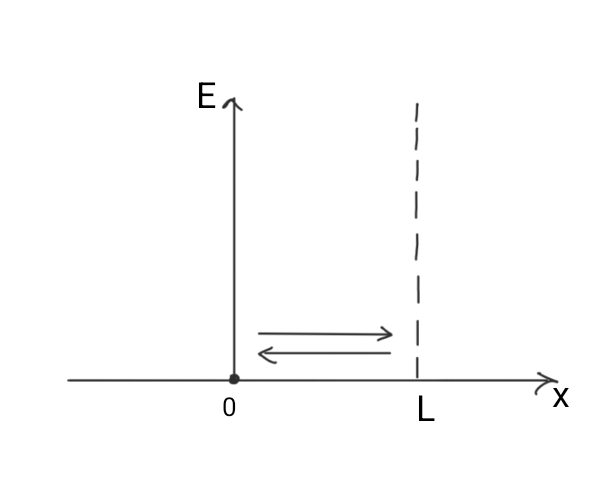
\includegraphics[height=5cm, width=7cm]{../img/kvantovy15.png}
\end{center}

\[A \cdot e^{i(kx+ \omega t)} = \psi_1\]
\[A \cdot e^{i(-kx - \omega t)} = \psi_2\]

Поскольку $e^{ikx} - e^{-ikx} = 2i \cdot \sin{kx}$

\[\Psi = \psi_1 + \psi_2 = A(e^{ikx} \cdot e^{-i \omega t} - e^{- ikx} \cdot e^{-i \omega t}) = A \cdot e^{-i \omega t} \cdot 2i \cdot \sin{kx} \]

Так как $\sin{kL} \Rightarrow kL = \pi n$ выведем формулу волного числа:
\[k = \frac{\pi n}{L} , n = 1, 2, \ldots\]
\begin{center}
    где n - количество длин волн
\end{center}

\textbf{Формула, определяющая длину волны:}
\[k = \frac{2 \pi}{\lambda}\]

Используя формулу Де-Бройля 
\[\lambda = \frac{\hbar}{mv} = \frac{\hbar}{p} \Rightarrow p = \frac{\hbar}{\lambda} = \frac{2 \pi}{\lambda} \cdot \frac{\hbar}{2 \pi} = k\cdot \frac{\hbar}{2 \pi}\]

\[\frac{\hbar}{2 \pi} = \hbar\]
\begin{center}
    --- \textbf{приведенная постоянная Планка}
\end{center}

Тогда:
\[p = \frac{n \cdot \hbar}{2 L}\]

Рассмотрим потенциальную энергию:
\[W = \frac{p^2}{2 m} = \frac{n^2 \cdot \hbar^2}{8L^2 m}\]
В силу того что $n \in \mathbb{Z}$, то $W$ принимает фиксированные значения - квантуется.

Рассмотрим атом водорода: пусть на электрон действует сила Кулона, а именно
\[F = \frac{1}{4 \pi \epsilon_0} \cdot \frac{q_e \cdot q_p}{r^2} = \frac{1}{4 \pi \epsilon_0} \cdot \frac{e^2}{r^2}\]
Рассмотрим второй закон Ньютона:
\[F = ma \Rightarrow a = \frac{v^2}{r} \Rightarrow\]
\[\frac{1}{4 \pi \epsilon_0} \cdot \frac{e^2}{r^2} = m \cdot \frac{v^2}{r} \Rightarrow\]
\begin{equation} \label{eq:r}
    r = \frac{e^2}{4 \pi \epsilon_0 m v^2}
\end{equation}

На орбиту электрона укладывается целое число волн, то есть число квантуется: 
\[2 \pi r = \lambda \cdot n\]
\begin{equation} \label{eq:bohr}
    2 \pi r = \frac{\hbar \cdot n}{m v}
\end{equation}
Решим систему \eqref{eq:r}, \eqref{eq:bohr} с неизвестными $r$ и $v$:

\[
\begin{cases}
r = \dfrac{e^2}{4 \pi \epsilon_0 m v^2},\\[4pt]
r = \dfrac{h n}{2 \pi m v}.
\end{cases}
\]

\[
\begin{cases}
e^2 \cdot 2 \pi m v = h n \cdot 4 \pi \epsilon_0 m v^2,\\[4pt]
r = \dfrac{h n}{2 \pi m v}.
\end{cases}
\]

\[
\begin{cases}
e^2 \cdot 2 \epsilon_0 h n = e^2,\\[4pt]
r = \dfrac{h n}{2 \pi m v}.
\end{cases}
\]

\[
\begin{cases}
v = \dfrac{e^2}{2 \epsilon_0 h n},\\[4pt]
r = \dfrac{h^2 n^2}{\pi m e^2}.
\end{cases}
\]

\textbf{Уравнение Шредингера:}


\begin{center}
\(\displaystyle \psi = A \cdot e^{i(kx - \omega t)}\) - для одномерного случая.    
\end{center}



\begin{center}
    где k - волновое число, $\omega$ - угловая скорость(волновой вектор)
\end{center}
Если $\psi_1, \psi_2 \ldots \psi_n$ - 

\[r = \frac{n^2 h^2 \epsilon_0}{m e^2 \pi}\]
\[v = \frac{e^2}{2h \epsilon_0 n}\]

Получаем, что чем дальше электрон, тем медленнее он будет вращаться.

Тогда:
\[E_k = \frac{mv^2}{2} = \frac{me^4}{8h^2 \epsilon_0^2 n^2}\]
\[E_p = \frac{1}{4 \pi \epsilon_0} \cdot \frac{e^2}{r} = - \frac{m e^4}{4 h^2 \epsilon_0^2 n^2}\]

Поскольку $\vec F = - \nabla E_n$ получаем полную энергию электрона на орбите при $E_n \to 0$ и $r \to \infty$:

\[E = E_k + E_p = - \frac{me^4}{8 h^2 \epsilon_0 ^2 n^2}\]

Электрон как и всякое тело стремится к минимуму потенциальной энергии, для электорна это достигается на нижней орбите --- самой стабильной орбите. 
Следовательно, электрон всегда стремится к нижней орбите, при этом он должен избавится от избытка энергии. 
Поскольку энергия электрона квантована, при переходе он испускает волны определенной частоты.
Причем этот набор у каждого элемента фиксирован. 

Свободный электрон может иметь любую энергию, а несвободный только фиксированную.
Будем называть валентным тот электрон, который прикрепленным к некоторому ядру, а свободным соответсвенно неприкрепленным.

\subsection{Энергетические состояния электронов в многоэлектронных атомах}

\subsubsection{Принцип Паули}
\begin{center}
    \textbf{\textit{В пределах одной квантовой системы в данном квантовом состоянии может находится только один фермион(электрон)}}
\end{center}
Квантовое состояние описывает всевозможное состояния квантовой системы, характеризуется \textbf{квантовыми числами.}
\begin {enumerate}
    \item n \textit{\underline{главное квантовое число} определеляет радус круговой орбиты или величину большой полуоси эллиптической орбиты.} (n = 1,2,3...)
Состояние электрона определяемое главным квантовым числом называют \underline{главным энергетическим уровнем.}

    \item l \textit{\underline{главное орбитальное квантовое число} определяет величину малой полуоси эллиптической орбиты.} (l = 0,1,2, \ldots n-1) 

    \item m \textit{\underline{магнитное квантовое число} (m = 0 +- 1... +- l) определяет ориентацию орбит, орбитальный магнитный момент электрона}

    \item s \textit{\underline{спиновое} квантовое число} s = +-1/2
\end{enumerate}

Из принципа Паули вытекает что на орбите не может находится не более двух электоронов.

\subsubsection{Принцип Хунда}
\begin{center}
    \textbf{\textit{Суммарное значение спина электронов данного подуровня должно быть максимальным.}}
\end{center}
\begin{center}
    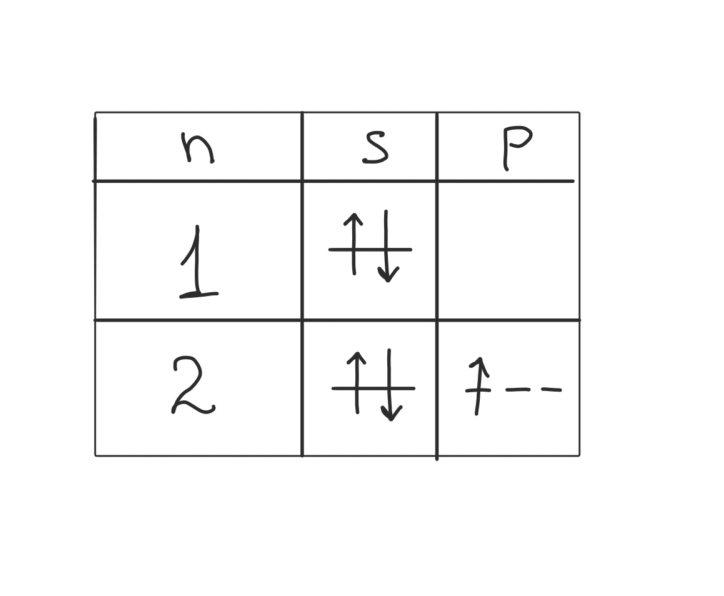
\includegraphics[height=5cm, width=7cm]{../img/kvantovy17.png}
\end{center}
\begin{center}
    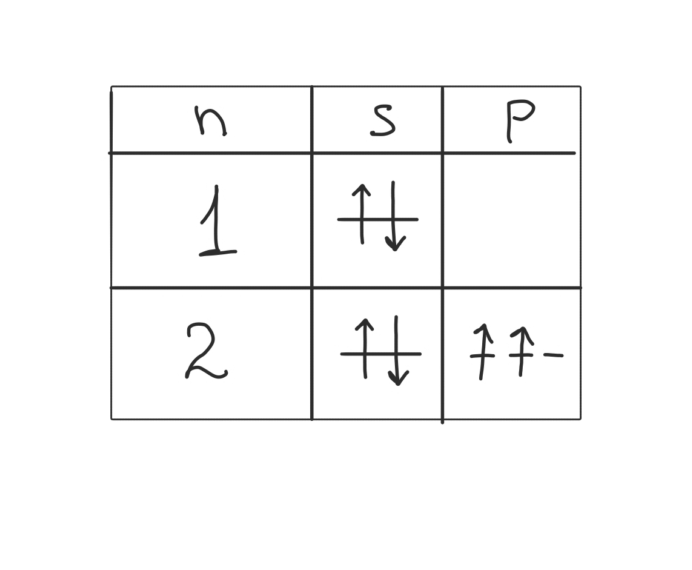
\includegraphics[height=5cm, width=7cm]{../img/kvantovy18.png}
\end{center}
\begin{center}
    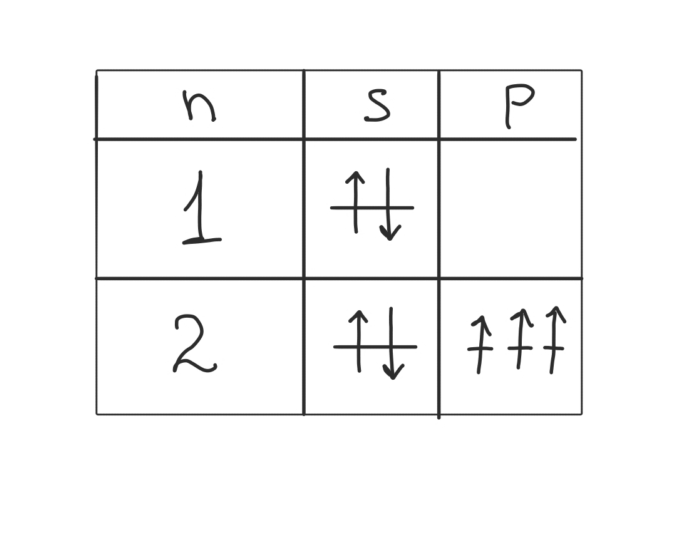
\includegraphics[height=5cm, width=7cm]{../img/kvantovy19.png}
\end{center}

\section{Виды химических связей}

\subsection{Ковалентная связь}

При такой связи возникает обоществленная пара электронов по одному от каждого атома. Различают два вида связи, связь \textbf{смещенная} и \textbf{несмещенная.}
\begin{center}
    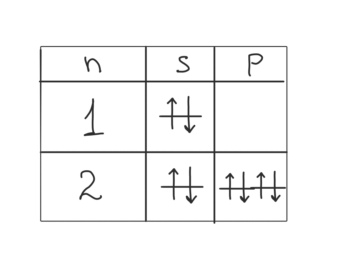
\includegraphics[height=5cm, width=7cm]{../img/kvantovy20.png}
\end{center}
\begin{enumerate}
    \item Несмещенная связь - возникает между атомами одинаковой массы($O_2, H_2, N_2$)
    \begin{center}
        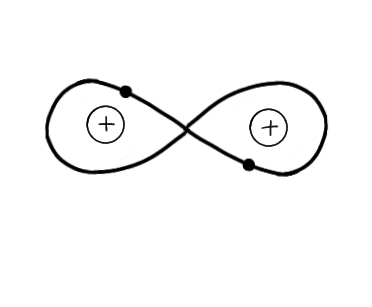
\includegraphics[height=5cm, width=7cm]{../img/kvantovy21.png}
    \end{center}
    \item Смещенная связь - обычно возникают между атомами с различным числом протонов в ядре, что вызывает \textit{поляризацию.}
    \begin{center}
        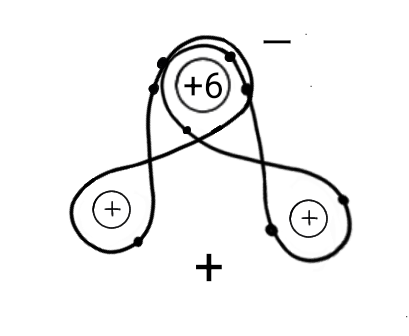
\includegraphics[height=5cm, width=7cm]{../img/kvantovy22.png}
    \end{center}
\end{enumerate}

\subsection{Металлическая связь}
Будем рассматривать решетку образованную электронами и ионами соотвесвтенно, такая решетка будет сохраняться за счет электронного облака.
\begin{center}
    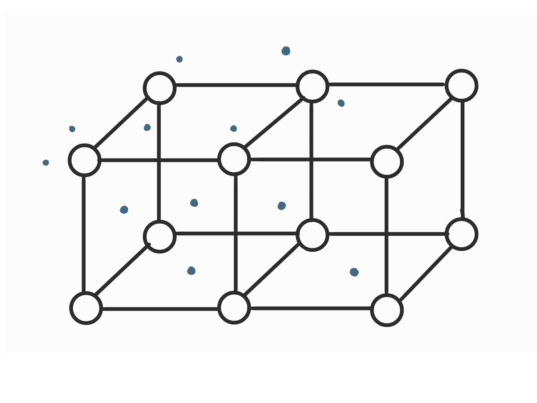
\includegraphics[height=5cm, width=7cm]{../img/kvantovy1.png}
\end{center}
\subsection{Ионная связь}
Характерно для связи металлов с неметаллами.
\begin{center}
    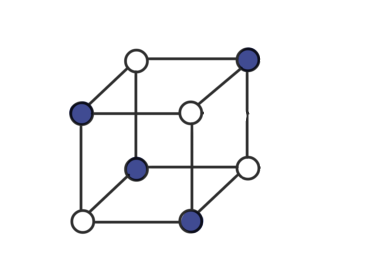
\includegraphics[height=5cm, width=7cm]{../img/kvantovy3.png}
\end{center}
\subsection{Молекулярная связь}
Возникает в газах при очень низких температурах.
\begin{center}
    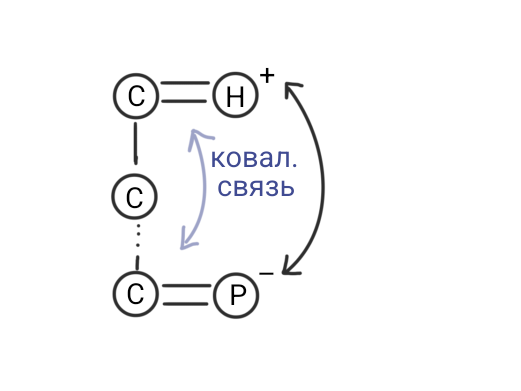
\includegraphics[height=5cm, width=7cm]{../img/kvantovy4.png}
\end{center}
\subsection{Водородная связь}

Для связь электрон может принимать фиксированное значение энергии, их называют энергетическими уровнями.

\section{Электопроводимость твердых тел}
Модель электронного газа - в металлах большое количество свободных электронов. Эти электроны внутри металла двигаются непрерывно и хаотично подобно молекулам газа.
При наличии электрического поля, эти свободные электроны приходят в упорядоченное движение, создавая электрический ток.

Напишем \textbf{среднюю хаотическую энергию электрона}:
\[E_t = \frac{3}{2} kT\]

В результате применения законов термодинамики приходим к этой формуле:
\[j = \frac{1}{\rho E}\]

Модель верна, потому что приходим потом к закону Ома в дифферернцированной форме.

При своем упорядоченном движении электроны сталкиваются с ионами кристаллической решетки, чем объясняется электрическое сопротивление. С ростом
температуры проводника увеличивается сопротивление проводника, поскольку само движение атомов становится активнее и электроны больше сталкиваются.

В полупроводниках наоборот: \textit{при уменьшении температуры увеличивается сопротивление}, то есть теория электронного газа \underline{не подходит} для полупроводников.

Сверхпроводимость  проявляется лишь при ультра низких температурах, на таком явлении построены квантовые компьютеры.

\section{Квантовая модель электропроводимости}
Рассмотрим энергию атомов, можно разделить на три уровня:
\begin{itemize}
    \item \textbf{Валентная зона} ($E_v$ - граница валентной зоны)
    \item \textbf{Запретная зона} --- те уровни энергии, которые не может принимать электрон в этом материале
    \item \textbf{Зона проводимости} --- электрон свободный и может перемещаться по материалу ($E_c$ - граница нижняя зоны)
\end{itemize}

\begin{center}
    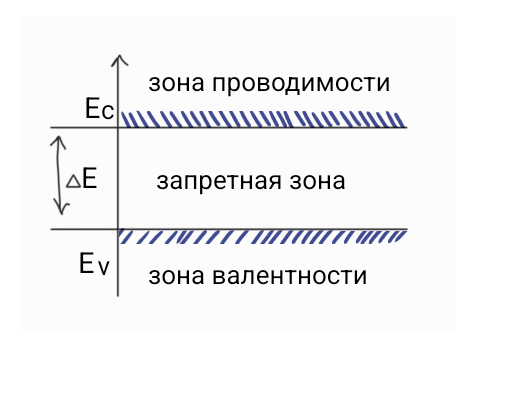
\includegraphics[height=5cm, width=7cm]{../img/kvantovy5.png}
\end{center}

Наивысшая плотность уровней в одной зона вблизи границ зон, верхней для валетной и нижняя для зоны проводимости.

\vspace{15px}

--- У металлов запретная зона практически отсутсутвует, $\Delta E < 0,1 $еВ - ширина запретной зоны, измеряется в энергиях эВ.

--- У полупроводников есть запретная зона, но $ 0,1 \leq \Delta E \geq 0,3$

--- У диэлектриков $\Delta E > 3 $

Чтобы перейти в другую зону, электрону нужно сообщить энергию, можно тепловую энергию(фотоэлементы).Для полупроводников 
достаточно сообщить тепловую энергию чтобы перевести в проводимое состояние. Для диэлектриков слишком широкая полоса для преодоления электронами, следовательно
не может идти ток, есть свободные электроны, но они не достигают зоны.

Для металлов, поскольку по сути запретной зоны нет то прееходя в другую зону они не вызывают такого влияния как колебания кристаллической решетки, следовательно 
сопротивление ухудшается.

\begin{center}
    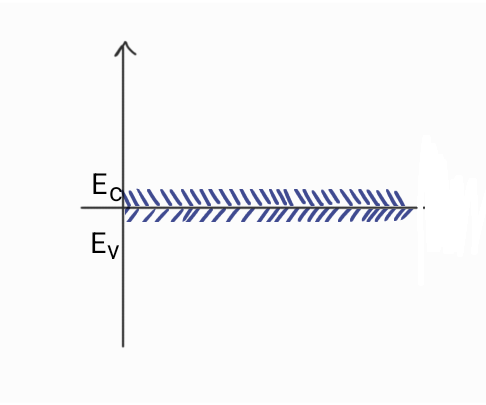
\includegraphics[height=5cm, width=7cm]{../img/kvantovy6.png}
\end{center}
\begin{center}
    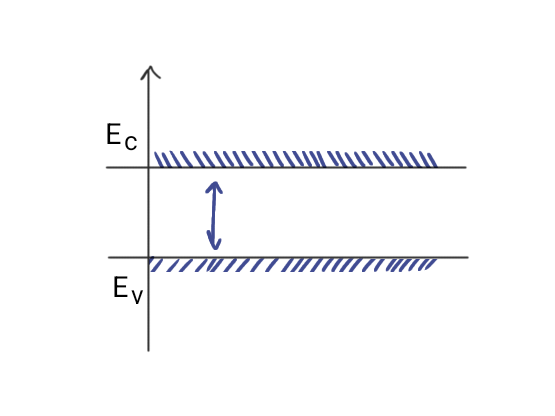
\includegraphics[height=5cm, width=7cm]{../img/kvantovy7.png}
\end{center}
\begin{center}
    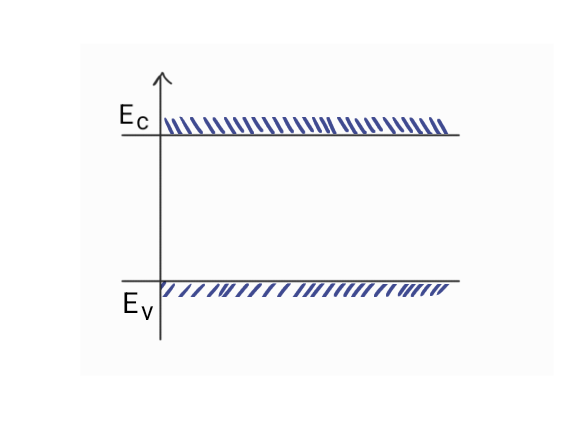
\includegraphics[height=5cm, width=7cm]{../img/kvantovy8.png}
\end{center}
Рассмотрим трехмерный потенциальный ящик, для одномерного: $P_p = \frac{h}{L} \cdot n \Rightarrow n = \frac{P_p}{h} \cdot L$, разложим квантовое число по каждому измерению: 
\[
\begin{cases}
n_x = \dfrac{2L}{h} \cdot P_x,\\[4pt]
n_y = \dfrac{2L}{h} \cdot P_y,\\[4pt]
n_z = \dfrac{2L}{h} \cdot P_z.
\end{cases}
\]


\[P^2 = P^2_x + P^2_y + P^2_z = \frac{h^2}{4L^2}(n_x^2 + n_y^2+n_z^2)\]

\[E = \frac{p^2}{2m} = \frac{h^2}{8mL^2}(n_x^2 + n_y^2+n_z^2)\]

\define Уровень Ферми - уровень энергии для которого заполненны электронные состояния  при T стремящемся к нулю называется уровнем энергии Ферми.

Для металлов $E_c = E_f = E_v$ это одна и та же линия. Вероятность обнаружить электрон на уровне Ферми = $\frac{1}{2}$

\textbf{Таким образом, уровень ферми определяет значение главного квантового числа.}

Тогда можем считать, что:
\[n_{zmax} = n_{ymax} = n_{xmax} = \frac{2L}{h} \cdot P_f\]

До сих пор мы рассматривали ящик в рассматриваемом пространстве, сейчас переходим к пространсву квантовых чисел, то есть 
по каждой оси число n ограниченно $n_max$

\[n = \sqrt{n^2_x+n^2_y+n^2_z} \leq \frac{2L}{h} \cdot P_F\]

\begin{center}
    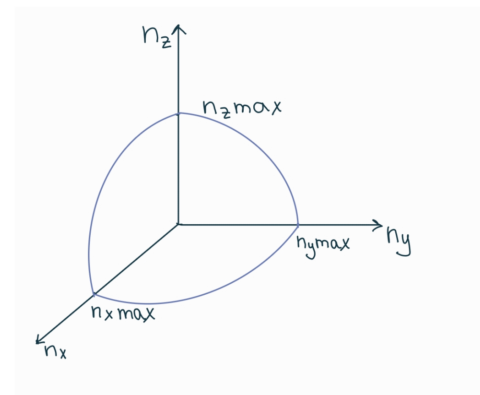
\includegraphics[height=5cm, width=7cm]{../img/kvantovy9.png}
\end{center}

Тем самым любое значение: 
\[0 < n_x, n_y,n_z \leq \frac{2L}{h} \cdot P_F\]
Определяет октант сферы, найдем площадь поверхности этой части сферы:

\[S = 2 \frac{1}{8} \frac{4}{3} \pi \cdot (\frac{2L}{h} P_F)^3 = \frac{8 \pi}{3} (\frac{P_F}{h})^3 \cdot L^3\]
\begin{center}
    где $L^3$ - объем потенциального ящика, обычно рассматривают в единице объема    
\end{center}

\[N = \frac{S}{V} = \frac{8 \pi}{3} \frac{P_F^3}{h^3}\]

\[P_F = \frac{h}{2} \cdot (\frac{3N}{\pi})^{\frac{1}{3}}\]

\[E_F = \frac{p^2}{2m} = \frac{h^2}{8m}(\frac{3N}{\pi})^{\frac{2}{3}}\]

\[N = \frac{\pi}{3} \frac{(8mE_f)^{3/2}}{h^3}\]

Найдем плотность энергетических состояний электрона на единицу энергии(количество состояний): 

\[\frac{dN}{dE} = \rho_N(E) = \frac{\pi (8m)^{\frac{3}{2}}}{2 h^3} \cdot E^{\frac{1}{2}}\]

\subsection{Распределение Ферми}
\begin{center}
    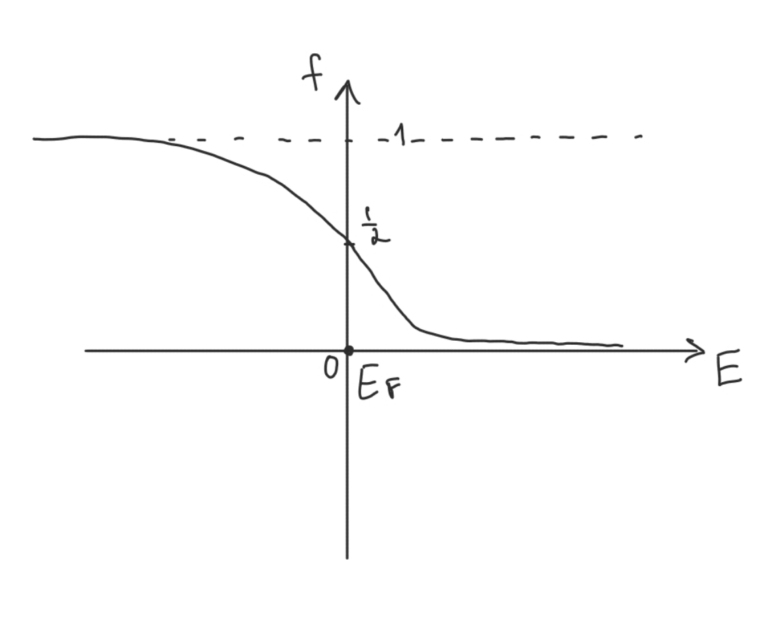
\includegraphics[height=5cm, width=7cm]{../img/kvantovy10.png}
\end{center}
Это функция f(E) представляет из себя вероятность того, что \textit{электрон будет находиться находится на данном уровне с энергией Е(вероятность заполнения состояния).}

\[f(E) = \frac{1}{1 + \exp{\frac{E-E_F}{kT}}}\]

Тогда концентрация электронов на данном уровне энергии:

\[h(E) = \rho_N(E) \cdot f(E)\]

Общая концентрация электронов:

\[n = \int_{E_F}^{\infty} f(E) \cdot \rho_N(E) dE\]

\subsection{Полупроводники}

Примеры полупроводников: кремний, германий, фосфор, мышьяк, сурьма

Ширина запрещенной зоны: Германий $\Delta E \approx 0,67$ Кремний $\Delta E \approx 1,12$

\subsubsection{Носители зарядов в полупроводнике}

\begin{center}
    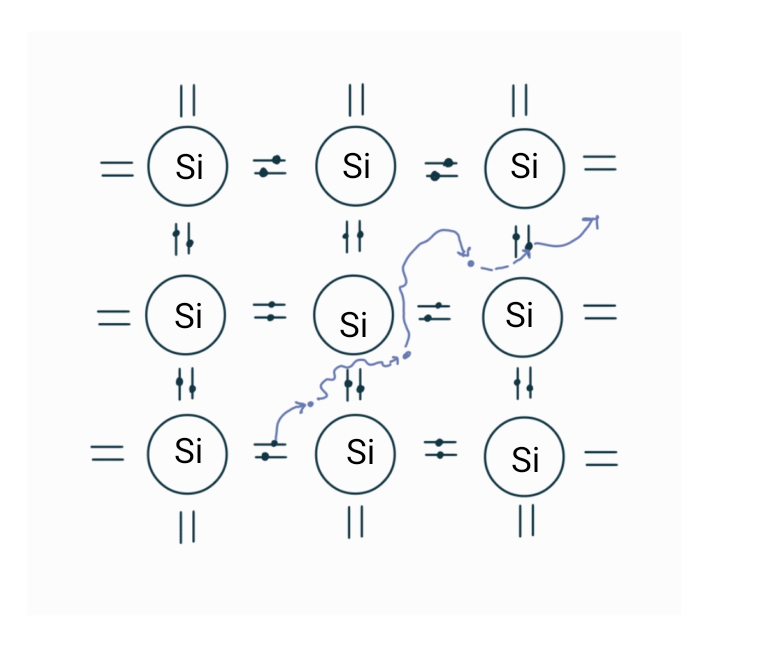
\includegraphics[height=5cm, width=7cm]{../img/kvantovy11.png}
\end{center}

Пусть электрон в решетке получает энергию чтобы выйти из ковалентной связи, следовательно из решетки - появляются свободные электроны.
Когда есть свободное место в связи(там меньше потенциальной энергии) он заходит туда.

Рассмотрим прошлое место, откуда ушел электрон, теперь оно свободно, там образуется положительный заряд, и так электрон может перейти на другую орбиталь с вакантным местом.
Так пустое место заряженное место перемещается до кристаллу, это место находится всегда в валентной зоне - поскольку меньше потенциальной энергии.

\begin{center}
    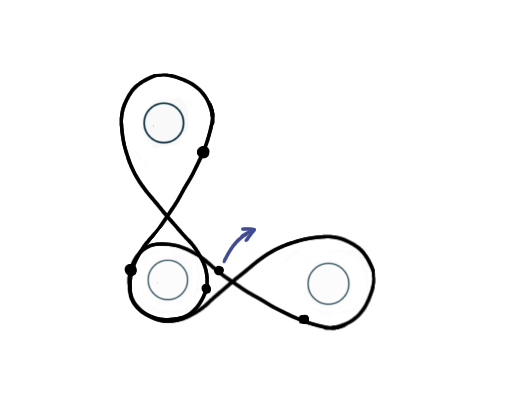
\includegraphics[height=5cm, width=7cm]{../img/kvantovy12.png}
\end{center}

В полупроводнике носители заряда являются как электроны так и вакантные места.(n - электрон, p - пустое место)
Так образуется пара - пустое место и электрон. 

В идеальном кристалле количество дырок и электронов совпадает.

Причем свободный и электрон в решетке это разные электроны и их массы не совпадают, у пустого места тоже есть масса называемая эффективной массой.

\begin{center}
    \(\displaystyle m^{*}_n = \frac{p_E}{v_n}\) --- масса электрона   
\end{center}

\begin{center}
    \(\displaystyle m^{*}_p = \frac{p_F}{v_p}\) --- эффективная масса   
\end{center}


\define Образование электронно-дырочной пары называется генерацией, обратный процесс - рекомбинацией. 
При генерации электрон из валентной зоны в зону проводимости, и при рекомбинации наоборот.

\vspace{15px}

Количество электронов в зоне проводимости:

\begin{center}
    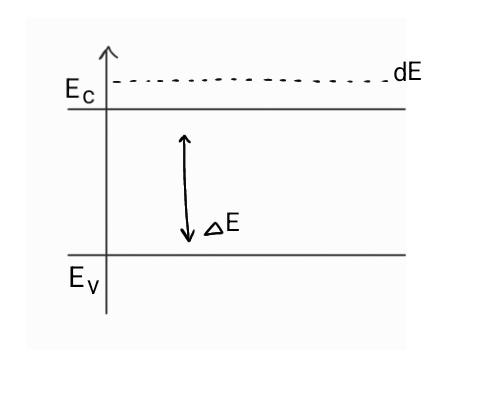
\includegraphics[height=5cm, width=7cm]{../img/kvantovy13.png}
\end{center}

\begin{center}
    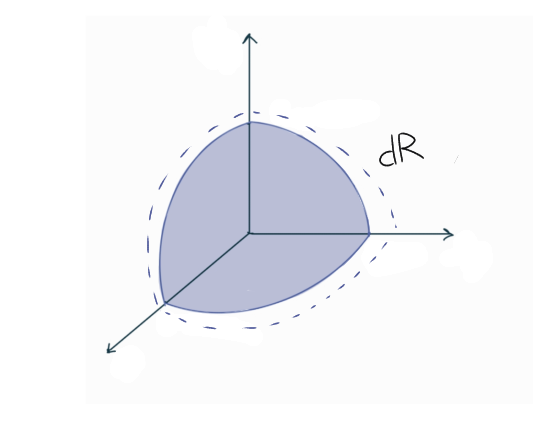
\includegraphics[height=5cm, width=7cm]{../img/kvantovy14.png}
\end{center}

\[R = \frac{2L}{h}p \Rightarrow dR = \frac{2L}{h}\cdot dp  \]
\[S = \frac{2}{8} \cdot 4 \pi R^2\]


\begin{center}
    \(\displaystyle V = \frac{2}{8} \cdot 4 \pi R^2 d R \Rightarrow = \frac{8 \pi L^3}{h^3} p^2 d p\) --- площать узкой области между $d E$ 
\end{center}

\[N = \frac{8 \pi}{h^3} p^2 d p\]

Общая энергия в полупроводнике
\[E = E_c + \frac{p^2}{2m_n}\]

Получим зависимость p от энергии и потом зависимость n:

\[p =  (2m_n(E-E_c))^\frac{1}{2}\]

\[d p  = \frac{\sqrt{2m_n \cdot dE}}{2(E - E_c)^{\frac{1}{2}}}\]
Тогда получим:

\[N = \frac{8 \pi}{h^3} \cdot 2m_n(E-E_c) \cdot \frac{\sqrt{2m}}{2} \cdot (E-E_c)^1/2 dE = \frac{4 \pi}{h^3}(2m_n)^{3/2} (E-E_c)^1/2 dE\]

\[ \frac{dN}{dE} = \rho\]
\[\rho_n(E) = \frac{4 \pi}{h^3}(2m_n)^3/2 (E-E_c)^1/2\]
\[\rho_p(E) = \frac{4 \pi}{h^3}(2m_p)^3/2 (E_v-E)^1/2\]

\[n = \int_{E_c}^{\infty} \rho_n(E) f(E) dE = \int_{E_c}^{\infty} \frac{4 \pi}{h^3}(2m_n)^3/2 (E-E_c)^1/2 \cdot \exp{\frac{- E - E_F}{kT}} dE\]
\[\frac{4 \pi}{h^3}(2m_n)^3/2 \int_{E_c}^{\infty} (E-E_c)^1/2 \cdot \exp{\frac{- E_c - E_F}{kT}} d E \Rightarrow \]

\[\frac{4 \pi}{h^3}(2m_n)^3/2 \cdot\exp{\frac{- E_c - E_F}{kT}} \int_{0}^{\infty} \sqrt{U}exp(-u) \cdot (kT)^3/2 = \frac{\sqrt{\pi}}{2} \]

Для полупроводников известно, что: 

\[E_c - E_f >> kT\]
\[E_F - E_v >> kT\]

$N_v$ --- \textbf{эффективная плотность состояний в валентной зоне}

Введем параметр n --- температурную концентрацию носителей заряда:

\[
\boxed{
n_i^2 = n \cdot p \Rightarrow 
n_i = \sqrt{N_c \cdot N_v} \cdot 
\exp\!\left(\frac{- \Delta E}{2 k T}\right)
}
\]

Рассматриваем температуру близкой к нулю градусов кельвина.

\subsection{Уровень Ферми в собственном полупроводнике}
\begin{center}
    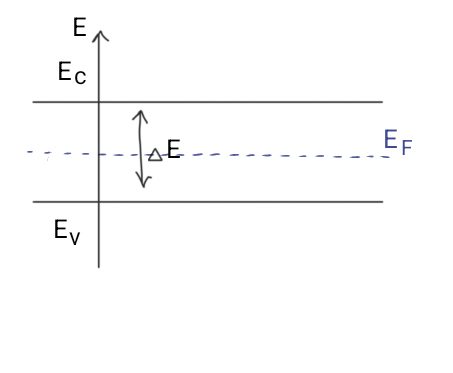
\includegraphics[height=5cm, width=7cm]{../img/kvantovy24.png}
\end{center}
Рассмотрим температуру стремящуюся к нулю градусов кельвина, скажем что веротяность появления электрона в зоне проводимости равна вероятности его отсутсвия в валентой зоне:
\[f(E_c) = 1 - F(E_v) \Rightarrow \frac{1}{1+ \exp{\frac{E_c - E_v}{kT}}} = 1 - \frac{1}{1+ \exp{\frac{E_v - E_f}{kT}}} \]
\[ = \frac{\exp{\frac{E_v- E_f}{kT}}}{1 + \exp{\frac{E_v - E_f}{kT}}} = \frac{1}{\exp{- \frac{E_v - E_f}{kT}} +1 } = \frac{1}{1+\exp{\frac{E_v - E_f}{kT}}}\]

Из монотонности функции F должны быть равны и агрументы функции то есть $\frac{E_c - E_v}{kT} = \frac{E_v - E_f}{kT}$, тогда получим:
\[E_f = \frac{E_c + E_v}{2}\]

Так уровень ферми располагается по центру и не зависит от температуры, он зафиксирован.

Представим что в решетке можно подставить в решетку атом другого элемента например атомо кремния, для того чтобы увеличить проводимость полупроводника.
Например, возьмем полупроводники Si, Ge. При легированнии проводников вносятся \textit{элементы третьей группы например In Ga} \textit{либо элементы пятой группы P As Sb.}
\begin{center}
    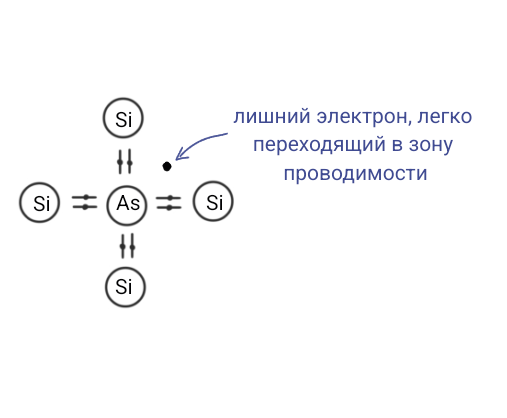
\includegraphics[height=5cm, width=7cm]{../img/kvantovy25.png}
\end{center}
Соотвественно получаем по свойствам разные полупроводники, так элементы 3 группы называются \textbf{акцепторами} 5 группы --- \textbf{донорами.}

\begin{itemize}
    \item Рассмотрим легирование элементами 5 группы
    Электрон не участвующий в связях разрывается и переходит в зону проводимости, получается от каждого атома донора внедренного в решетку мы получаем свободный электрон $\Rightarrow$ получается мы существенно 
увеличиваем количество свободных электронов $\Rightarrow$ количество дырок резко уменьшается, тогда $n >> p n * p = n^2$ 
\begin{center}
    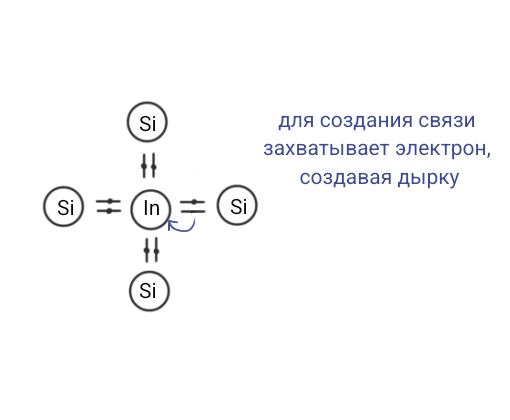
\includegraphics[height=5cm, width=7cm]{../img/kvantovy26.png}
\end{center}
\define Такой полупроводник называется \textit{полупроводником с электронной проводимостью} или \textit{полупроводник n-типа.}

--- $N_D$ --- концентрация доноров в примеис, каждый атом вносит в полупроовдник свободный электрон.

--- $n_n = N_D +p_n$ --- соотношения связи между электронами и дырками в полупроводника n-типа
 Таким образом концентрация электронов примерно равняяется концетрации доноров.

    \item Рассмотрим легирование акцепторами
    Например, помещаем индий (3 группа).
    Так на одной из связей будет вращаться один электрон, то есть образуется дырка или вакантное место. Так будут поглащаться свободные электроны в эти дырки.
    Так $p >> n$, концетрация акцепторов $N_A$. 
    
\define Эти полупроводники называются \textit{полупроводниками с дырочной проводимосттью} или \textit{полупроводниками p-типа} $p_p = N_A + n_p$

\end{itemize}

\subsection{Уровень Ферми в легированных проводниках.}

Уровень ферми не двигается, двигаются только границы $E_c$ и $E_v$.

Рассмотрим изменения при легировании: 

\[ n_n = N_c \cdot \exp{-\frac{E_c - E_f}{kT}} \]
\[ p_n = N_v \cdot \exp{-\frac{E_f - E_c}{kT}} \]

Возьмем отношение $\frac{n_n}{p_n} = \frac{N_c}{N_v} \cdot \exp{- \frac{E_c + E_v - 2E_F}{kT}}$

Берем $\frac{N_c}{N_v} \approx 1$ 

Известно из $n_i^2 = n_n \cdot p_n \Rightarrow p_n = \frac{n_i^2}{n_n}$ подставим 
\[\frac{n_n^2}{n_i^2} = \exp{- \frac{E_c + E_v - 2E_F}{kt}}\]
\[2 \ln{\frac{n_n}{n_i}} = - \frac{E_c + E_v - 2E_F}{kt} \Rightarrow kT \ln{\frac{n_n}{n_i} = - \frac{E_c + E_v}{2} +E_f}\]

Для n-типа:
\[
\boxed{
E_f = \frac{E_c + E_v}{2}
- kT \ln{\frac{n_n}{n_i}}
= \frac{E_c + E_v}{2}
- kT \ln{\frac{N_D}{n_i}}
}
\]

Уровень ферми будет смещен ближе к зоне проводимости. Выше для p типа: 

\[
\boxed{
E_f = \frac{E_c + E_v}{2}
- kT \ln{\frac{p_p}{n_i}}
= \frac{E_c + E_v}{2}
- kT \ln{\frac{N_A}{n_i}}
}
\]

То есть уровень Ферми больше смещен к зоне проводимости.

\define Если уровень Ферми при легировании попадает в зону проводимости(для n типа) 
или в валентную зону (p - тип) такие полупроводники называются \textbf{вырожденными.}

\begin{center}
    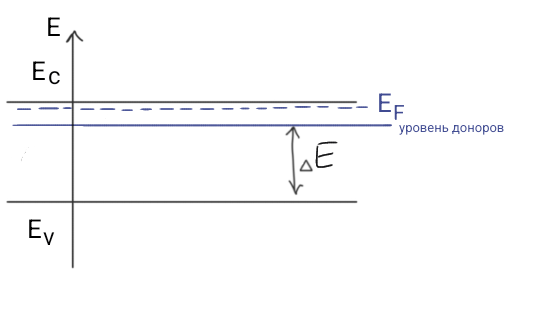
\includegraphics[height=5cm, width=7cm]{../img/kvantovy27.png}
\end{center}
\begin{center}
    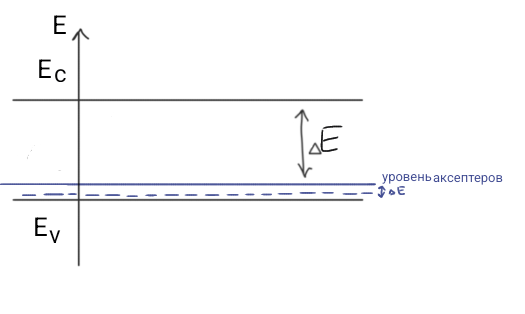
\includegraphics[height=5cm, width=7cm]{../img/kvantovy28.png}
\end{center}
По хорошему уровень Ферми должен распологаться в запретной зоне.



\subsection{Движение свободных носителей заряда в полупроводниках.}

В полупроводниках будем рассматривать движение не только из-за действия электрического поля, но из-за неравномерного распределения электронов из меньшей концентрации в большую.

\define Ток в полупроводнике модет быть вызван двумя причинами: при наличии электрического поля и такой ток называется \textbf{дрейфовый} и в следствии
 неравномерного распределения на сфере заряда --- \textbf{диффузионный.}

Мы будем рассматривать именно плотность тока:
\[j = q k v\]
\begin{center}
    --- плотность тока в проводника, v скорость направленного движения тока, за направление тока мы принимает движение положительных частиц.    
\end{center}

\subsubsection{Дрейфовый ток}

Рассмотрим движения дрейфовых электронов: электроны будут идти в одну сторону, а ток в другую соотвественно

\[j = -e \cdot n \cdot V\]

Вычислим подвижность электрона $\mu = \frac{v_n}{E} \Rightarrow v = - \mu E$. Эта подвижность характеризуется свойствами материалов. 

Тогда для электронов:

\[j = e \cdot n \cdot \mu_n E\] 

В выражении выше нет знака, поскольку ток движется в направлении электрического поля.

Для дырок:

\[j = e \cdot p \cdot \mu_p e\]

\textbf{Напомним: Закон Ома в диф форме $j = \frac{E}{\rho} \sigma = 1/\rho$}

\subsubsection{Диффузионный ток}

Диффузия это стремление вещества распространится по всему объему равномерно. Возникает тогда когда электроны и дырки распространенны неравномерно,
тогда возникает стремление заполнить объем равномерно, например с концентрацией k:

\[\Phi_k = -D_k \nabla k\]
\begin{center}
    --- D --- поток частиц через поверхность единичной площади через площадку в единицу времени.    
\end{center}


Перейдем к полупроводникам и рассмотрим плотность тока.
\[\vec j_{difn} = e \cdot D_n \cdot \nabla n = -e \cdot n \cdot \vec v_{difn} \]

\[\vec j_{difp} = - e \cdot D_p \cdot \nabla p = e \cdot p \cdot \vec v_{difp}\]

\[
\boxed{
\begin{aligned}
\vec{j}_n &= \vec{j}_{\mathrm{difn}} + \vec{j}_{\mathrm{drp}} = e\!\left(n \mu_n E + D_n \nabla n\right),\\[6pt]
\vec{j}_p &= \vec{j}_{\mathrm{difp}} + \vec{j}_{\mathrm{drp}} = e\!\left(p \mu_p E + D_p \nabla p\right).
\end{aligned}
}
\]

\subsection{Уравнение неразрывности}
\[\frac{d \rho_p}{d t} = - \mathrm{div}( \vec j)\]
\begin{center}
    --- изменение плотности заряда за время T --- \textbf{уравнение неразрывности}
\end{center}

Плотность заряда для электронов
\[\rho_{qn} = - e \cdot n\]
\[\deriv{-en}{t} = -\mathrm{div}(e \mu_n n \vec E + e D_n \nabla n)\]
\[-e \frac{d n}{d t} = -e \mu_n \mathrm{div}(n \vec E) - eD_n \Delta n\]

\[
\boxed{
\frac{d n}{d t} = \mu_n \, \mathrm{div}(n \vec{E}) + D_n \, \Delta n
}
\]
\begin{center}
\textit{Уравнение неразрывности для свободных электронов в проводнике.}
\end{center}

\[
\boxed{
\frac{d p}{d t} = \mu_n \, \mathrm{div}(p \vec{E}) + D_n \, \Delta p
}
\]
\begin{center}
\textit{Уравнение неразрывности для дырок в проводнике.}
\end{center}



При рассмотрении легированных проводников $n_n = N_D$, поэтому уравнение неразрывности мы рассматриваем для неосновных носителей зарядов.

Записываем с учетов генерации и рекомбинации:

\[\frac{d n_p}{d t} = \mu_n \frac{d n \vec E}{dx} + D_n \cdot \frac{d^2 n}{dx^2}+ G_n - \frac{n_p - n_p0}{\tau_n}\]

\[\frac{d p_n}{d t} = \mu_n \frac{d n \vec E}{dx} + D_n \cdot \frac{d^2 n}{dx^2}+ G_p - \frac{n_p - n_p0}{\tau_n}\]

\begin{center}
    \textit{Здесь: $G$ — скорость генерации электронов и дырок; $p, n$ — равновесные концентрации неосновных носителей заряда; 
    $\tau_n$ — характерное время рекомбинации (среднее время, в течение которого электрон остаётся свободным);}
    
    \textit{$\mu_n$ — подвижность электрона; $D_n$ — коэффициент диффузии.}
    \end{center}

\textbf{\textit{Соотношение Энштейна}}

\[
\boxed{
\begin{aligned}
D_n &= \frac{kT}{e} \, \mu_n, \\[6pt]
D_p &= \frac{kT}{e} \, \mu_p.
\end{aligned}
}
\]

\section{Электрические переходы}

\define \textit{\textbf{Электрический переход}} называется граничный слой между двумя областями, электрические характеристики которых имеют существенные физические различия.

\vspace{10px}

В полупроводниках 4 перехода:

\begin{enumerate}
    \item \underline{Электронно-дырочный} переход или $p_n$ переход
    Переход между двумя областями одного и того же полупроводника имеющими различный тип электропроводимости, но полупроводник один и тот же
    \item \underline{Переход металл-полупроводник}
    \item \underline{Переход между двумя областями проводника с одним типом электропроводимости}, 
    
    но с различной степенью легирования
    \item \underline{Гетеро-переход переход между двумя различными полупроводниковыми материалами}
    
    с различной шириной запрещенной зоны.
\end{enumerate}

\subsection{P-N переход.Контактные явления на границе}


Рассмотрим полупроводниковый переход типа \textit{p–n}. 
В начальный момент после его образования начинается \textbf{диффузия} электронов из \textit{n}-области в \textit{p}-область и дырок — из \textit{p}-области в \textit{n}-область. 
В результате диффузии вблизи границы раздела происходит \textbf{рекомбинация} носителей заряда. 
Из-за этого в приповерхностных слоях остаются оголённые ионы доноров и акцепторов, что приводит к \textbf{накоплению неподвижного заряда} и возникновению \textbf{внутреннего (контактного) электрического поля}.

Это поле создаёт разность потенциалов между областями:
\[
\Delta \varphi = \varphi_p - \varphi_n,
\]
которая называется \textbf{потенциальным барьером}.

Возникающее контактное поле препятствует дальнейшей диффузии носителей заряда. 
Однако носители, обладающие достаточной энергией, могут преодолеть барьер — их движение обусловлено диффузией и формирует \textbf{диффузионный ток}. 
Для основных носителей заряда это поле не является препятствием: они перемещаются под действием поля, создавая \textbf{дрейфовый ток}.

В конце концов устанавливается \textbf{динамическое равновесие}, при котором диффузионный ток неосновных носителей полностью компенсируется дрейфовым током основных носителей. 
В области перехода формируется \textbf{запирающий слой}, лишённый подвижных носителей заряда, внутри которого существует \textbf{контактное электрическое поле}.


\define Если $N_A \approx N_D$ то такой переход называют \textit{симметричным} переходом, иначе \textit{несимметричным.} 

Более высокая степень легирования области обозначается плюсом: $n^{+}, p^{+}$


\section{Тест 1}

\subsection{Задание 1}
\begin{itemize}
    \item Длина волны Де Бройля обратно пропорциональна импульсу частицы ($\lambda = h/p$, где $\lambda$ -- длина волны, $h$ -- постоянная Планка, а $p$ -- импульс частицы)
    \item Гипотеза Де Бройля состояла в предположении о наличии волновых свойств микрочастиц.
    \item Любой частице, обладающей импульсом $p$ можно сопоставить волновой процесс с длиной волны $h/p$. ??? Вар 3
    \item Длина волны Де Бройля обратно пропорциональна массе частицы и ее скорости ($\lambda = h/p = h/mv$, $p = mv$, где $m$ -- масса частицы, $v$ -- скорость частицы.)
    \item Движение любой элементарной частицы с массой $m$ и скоростью $v$ описывается $\lambda = h/mv$.
\end{itemize}

\subsection{Задание 2}
\begin{itemize}
    \item Что выражают соотношения неопределённости в квантовой механике? -- Соотношения между погрешностями координатами и импульсами микрочастицы, а также между погрешностями энергией микрочастицы и моментом времени.
    \item Соотношение неопределённостей Гейзенберга для проекций импульса и координаты говорит о том, что одновременное точное определение координаты и проекции импульса частицы невозможно.
    \item Из соотношения Гейзенберга следует, что при уменьшении неопределённости импульса частицы, неопределённость в её координате возрастает. ($\Delta x \cdot \Delta p \ge h/2$, где $\Delta x$ -- неопределённость положения частицы, $\Delta p$ -- неопределённость импульса частицы)
    \item Из соотношения Гейзенберга следует, что при уменьшении неопределённости энергии частицы неопределённость в моменте времени возрастает. ($\Delta E \cdot \Delta t \ge h$, где $\Delta E$ -- неопределённость энергии, а $\Delta t$ -- промежуток времени, в течение которого это состояние существует. $\Delta t \ge h/\Delta E$)
\end{itemize}

\subsection{Задание 3}
\begin{itemize}
    \item Если частица $\psi$ может быть в состоянии $\psi_1$ и $\psi_2$, то общее состояние частицы описывается волновой функцией $\Psi = c_1 \Psi_1 + c_2 \Psi_2$, где $c_1$ и $c_2$ -- некоторые константы (согласно принципу суперпозиции)
    \item Вероятность обнаружить частицу в указанной точке пространства в данный момент времени пропорциональна квадрату модуля волновой функции.
\end{itemize}

\subsection{Задание 4}
(Радиус орбиты электрона пропорционален квадрату номера орбиты. Скорость движения электрона по орбите обратно пропорциональна номеру орбиты -- для первой орбиты она равна $2,186 \times 10^6$ м/сек, для второй -- $1,093$.
Электрон излучает энергию (фотон), когда переходит с более высокого энергетического уровня на более низкие. При обратных переходах электрон, наоборот, поглощает энергию. Энергия не меняется, когда он находится на стационарной орбите)

\textbf{Верные утверждения:}
\begin{itemize}
    \item Разрешёнными орбитами для электронов являются те, длина которых пропорциональна (кратна) длине волны электрона.
    \item В атоме существуют стационарные состояния, когда энергия не изменяется во времени без внешних воздействий.
    \item Радиус орбиты электрона не может измениться без внешнего воздействия.
\end{itemize}

\textbf{Неправильные утверждения:}
\begin{itemize}
    \item При переходе на другую орбиту энергия не меняется.
    \item Электрон в атоме водорода обладает максимальной энергией на ближней от ядра орбите.
    \item При переходе электрона с ближней орбиты на дальнюю его скорость увеличивается.
\end{itemize}

\subsection{Задание 5}
\begin{itemize}
    \item Из принципа Паули следует, что количество электронов на каждом уровне может быть не более двух. (ни одна пара электронов в атоме не может иметь одинаковые электронные квантовые числа)
    \item На одной орбите любого атома может находится не более двух электронов.
    \item В квантово-механической системе в данном квантовом состоянии может находится не более 2 электронов.
\end{itemize}

\subsection{Задание 6}
\begin{itemize}
    \item Главное квантовое число характеризует энергетический уровень электрона.
    \item Орбитальное квантовое число характеризует ориентацию эллиптической орбиты в пространстве.
    \item Магнитное квантовое число характеризует ориентацию эллиптической орбиты в пространстве. (Оба числа, орбитальное ($l$) и магнитное ($m_l$), связаны с ориентацией орбитали в пространстве, но на разных уровнях.)
    \item Спиновое квантовое число характеризует собственный магнитный момент электрона.
\end{itemize}

\subsection{Задание 7}
\begin{itemize}
    \item Спиновое квантовое число для электрона может принимать значения: $s = \pm 1/2$.
    \item Магнитное квантовое число в состоянии с орбитальным квантовым числом 1 может принимать значения: $m = 0, \pm1, \pm2, \dots, \pm l$.
    \item Главное квантовое число является: натуральным числом ($n = 1, 2, 3, \dots$)
    \item Какие значения может принимать орбитальное квантовое число с главным квантовым числом $n$? $l = 0, 1, 2, \dots, n-1$ (т.к. $n$ определяет форму орбитали)
\end{itemize}

\subsection{Задание 8}
\begin{itemize}
    \item Химическая связь, возникающая при взаимодействии ионов решётки с электронным газом – металлическая связь
    \item Химическая связь, возникающая за счёт обобществления электронной пары – ковалентная связь
    \item Химическая связь, обусловленная кулоновским взаимодействием противоположно направленных ионов – ионная связь
    \item Химическая связь, возникающая при взаимодействии газовых молекул при низких температурах – молекулярная связь
    \item Нет в варианте, но есть в ответах: Ковалентная связь – это химическая связь, образованная за счёт образования общей электронной пары у двух атомов вещества при сближении их ядер.
\end{itemize}

\subsection{Задание 9}
\begin{itemize}
    \item Ширина запрещённой зоны твердотельного материала характеризует минимальную энергию, необходимую для перевода электрона из валентной зоны в зону проводимости.
    \item Уровень Ферми -- энергетический уровень, до которого заполнены электронные состояния при $T = 0$K.
    \item Согласно теории электронного газа электрическое сопротивление объясняется соударениями электронов с узлами кристаллической решётки.
    \item 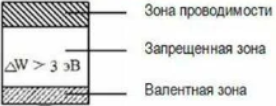
\includegraphics[width=5cm, height=2cm]{../img/test1_9.png}
\end{itemize}

\subsection{Задание 10}
\begin{itemize}
    \item Согласно квантовой теории проводимости различие между диэлектриками, полупроводниками и проводниками состоит в ширине запрещённой зоны.
    \item В порядке убывания ширины запрещённой зоны вещества располагаются: диэлектрик, полупроводник, металл.
    \item В порядке возрастания энергии, необходимой для перехода электрона из валентной зоны в зону проводимости, вещества располагаются: металл, полупроводник, диэлектрик.
\end{itemize}
\end{document}
